\documentclass[a4paper,12pt,titlepage]{report}
\usepackage{listings}
\usepackage{color}

\lstset{language=Java, keywordstyle=\color{blue}, breaklines=true, captionpos=b, showspaces=false}

\usepackage{graphicx}

\DeclareGraphicsExtensions{.pdf,.png,.jpg}
\graphicspath{ {images/}}

\title{Matygo: a Modern Classroom Support System}
\author{William Joseph Gaudet SID:12919098}
\linespread{1.5}
\begin{document}
\maketitle

\newpage
\tableofcontents
\newpage

\begin{abstract}
The purpose of this document is to provide an architectural overview of the Matygo Learning Management System - a next generation classroom support system developed in part while the author was attending the University of British Columbia (UBC).
The Matygo LMS is composed of 5 principle components: a web based application programming interface (API) code named Aristotle; a rich JavaScript single page load client named Darkhorse which targets the desktop web browser; an iOS mobile Application named Socrates; an android mobile Application (retroactively named: Aristophanes);  and a Ruby on Rails client named Plato. 
In addition to detailing each of these systems and their interactions, some consideration will be given to over all system operations (ops) and deployment schemes.
\end{abstract}

\section{Introduction} % (fold)
\label{sec:introduction}

\subsection{Motivation} % (fold)
\label{sub:motivation}

Matygo was founded by William Joseph Gaudet (MASCEng Student) and Paul Roland Lambert (BCS) while attending UBC in 2009. 
Originally conceived as a tutor marketplace with the goal of connecting struggling students with available tutors based on recommendations, Matygo struggled to find a large user base due to a lack of tutors for students to choose from which in turn made the system unappealing to prospective tutors.
To address this chicken and the egg problem, as well as a growing dissatisfaction with the existing LMS named Blackboard (discussed in section \ref{sub:state_of_the_art}) the founders set out to create the LMS described in this document. 
Over 2000 students logged into the Matygo LMS daily from 7 schools in the lower mainland of British Columbia, however it was designed to easily scale to a much wider audience.
% subsection motivation (end)

\subsection{State of the Art} % (fold)
\label{sub:state_of_the_art}

When Matygo broke ground on the LMS project, UBC was using the Blackboard LMS. 
At this point a largely antiquated system, which required client side Java applets in order to handle various features, including assignment submission (a feature which was sufficiently difficult to use the computer science department opted to use their in house handin solution).
Furthermore, the Blackboard LMS required a centralized installation on custom hardware within the firewall of the Universities using the systems.
These architecture choices gave rise to glacial upgrade cycles (in the order of multiples of years), and prevented students from using the increasingly popular mobile platforms such as the iPhone or the Android systems, as neither support Java applets in their respective browser implementations.

% subsection state_of_the_art (end)

\subsection{Requirements} % (fold)
\label{sub:requirements}

Requirements for the Matygo LMS were gathered during interviews with a variety of professors from UBC in the Electical and Computer Engineering (ECE) and Computer Science (CS) departments. They are enumerated here for the purpose of scope, specific implementation details at the feature level will not be given.

\begin{itemize}
	\item Authentication and Role Based Authorization - in conjunction with UBC's campus wide login. 
	\item Notifications - configurable notifications for a variety of system events via email.
	\item Discussion Board - a fully featured discussion board with LaTeX typesetting system included. 
	\item Grade Book - for grading and delivering grades to students.
	\item Assignments - a system of delivering assignments 
	\item Learning Materials - a general purpose container for delivering various learning assets (PDFs, Videos, Presentations)
	\item Security - connections must be secure, additional any Canadian student records must be stored on Canadian soil 
\end{itemize}

These requirements evolved over time to include real time updates to the clients, user to user messaging, and assignment submission. All features which did not make it past the alpha stages before Matygo pivoted the business into a public and then corporate education spaces. 

% subsection requirements (end)

% section introduction (end)

\section{Aristotle} % (fold)
\label{sec:aristotle}

The Aristotle webservice provides an unified interface to all of the data resources in the Matygo LMS, these include structured data stored in the MySQL database, resource metadata (also stored in MySQL), and resources (uploaded files, images, etc.).A

Its primary responsibility is to provide role authorized access and mutation of these resources and metadata. It also handles system event notification as well as nightly digest notification.

During the service life of the Aristotle API, it was re-designed twice, once to switch out persistence engines from Cassandra to MySQL, and again to change out the implementation language from Java to Scala.

\subsection{Representational State Transfer} % (fold)
\label{sub:rest_webservices}

The central architectural design is based on a the Aristotle WebService API is Representational State Transfer or REST design. The REST standard was developed along side of HTTP 1.1, based on the work of Roy Fielding [CITATION NEEDED].
In REST any resource in a system has a uniform resource identifier (URI), and can be accessed and mutated by way of the various HTTP request methods. 
REST becomes particularly useful in creating create read update destroy (CRUD) services as its semantics map directly to those common database actions. 
Additionally by following the conventions of REST, one can more easily leverage existing client libraries when targeting new platforms. Additionally if implemented properly, a REST api can easily leverage the existing wide spread HTTP infrastructure, particularly with respect to cacheing.

The following trivial example of REST will serve to illustrate how such an architecture simplifies implementation of clients as well as overall system semantics.

\begin{table}
\begin{center}
\begin{tabular}{ | c | c | c | }
\hline
URI & HTTP Method & REST Action \\ \hline
/assignments & GET & Index \\ \hline
/assignments/:id & GET & Show \\ \hline
/assignments/:id & PUT & Update \\ \hline
/assignments/:id & DELETE & Destroy \\ \hline
/assignments & POST & Create \\ \hline
/assignments/:id/submissions & POST & Custom \\ \hline
/assignments/:id/custom & POST & Custom \\ \hline
\end{tabular}
\end{center}
\caption{Common mappings of HTTP request and URIs to REST actions.}
\label{tab:rest_actions}
\end{table}


Suppose we had a resource from our LMS, an assignment, we would implement the  endpoints shown in Table~\ref{tab:rest_actions} in the API (Assuming a base URI of https://api.matygo.com/v1).
As we can see REST crud actions map nicely to the HTTP request methods.
The use of a unique URI coupled with the request methods provides a simple and consistent interface (note: the :id specifier is the unique key required to look up the resource - this is usually a monotonically increasing integer but could be any system wide unique key.
Consider if the resource was instead announcements, only the URI would have to change (from assignments to announcements) and all the semantics would remain the same.

Requests which use the GET method should be side effect free, making no change to the resource, while requests that use either the PUT or DELETE methods are required to be idempotent.
Custom actions are usually mapped to the POST request method, with the URI taking on an additional path parameter of the action the caller wishes to take - in our assignments example an assignment submission might take the form of a POST to /asssigments/:id/submissions with a payload of the assignment either as post data or as some JSON content. 

It should be noted that there must be an additional consideration for the Internet Media Type which should be used to represent the resource. 
Usually this is done by way of specifying the format in an extension - eg: /assignments becomes /assignments.json for JSON or /assignments.xml for XML - however in Aristotle the media type is set by way of the HTTP accept header.


% subsection rest_webservices (end)

\subsection{The JVM, Java, and Scala} % (fold)
\label{sub:jvm}

The initial implementation of Aristotle was on the Java Virtual Machine (JVM) written in Java on a Jetty WebServer [CITATION NEEDED]. 
Java was originally selected by Matygo for its large number of free and open source libraries which decreases the time required for implementing features considerably.
Additionally when compared with other WebServers / Frameworks the embedded Jetty system is considerably simpler to deploy and operate. 
To do so, one simply creates an executable Java archive file (JAR) and runs it on the target server.

However, after initial development the verbosity of Java started to hamper maintainability. Due to the lack of first order functions, actions as simple as extracting items from a list require at least 5 lines of code. 
Additionally, Jetty's routing configuration and dispatch mechanisms are not very sophisticated. 
For instance if you wish to add an endpoint to a Jetty WebService, you must configure it using the loathsome Web.xml - which allows you to point a wild card route at a particular Java Servlet [CITATION OF SERVLET API].
That servlet must handle dispatching based on the URI and method of the Request.
We had initially developed a meta routing mechanism for handling this configuration problem.
Where by each handler method would be annotated with a method and a regular expression used to match the URI as shown in Listing \ref{list:java_annotation}. 
This method required a complicated compile step which would generate the web.xml file. We eventually abandoned this process in favor of Scala and the Scalatra web framework.
\begin{lstlisting}[caption=Java Annotated Method Handler, label=list:java_annotation]
public class CourseServlet extends HttpServlet {
	@route{method=Methods.GET, path="/courses"}
	public String coursesIndex(HttpServletRequest req, HttpServletResponse res){
		return "Hello World";
	}
}
\end{lstlisting}

Scala is arguably one of the more popular JVM hosted languages, developed by Martin Odersky in order to address some of the shortcomings of the Java programming language, it was chosen due to its first class functional support, Java interoperability, and general code maintainability. 
Take our example from Listing \ref{list:java_annotation}, refactored in Scala using the Scalatra WebFramework (which is still hosted by embedded Jetty) our code looks much more tidy and intent revealing. 
This choice has continued to pay dividends as Java continues to languish in the JSR committees [CITATION NEEDED], Scala adds new features regularly allowing Matygo to leverage this work.

\begin{lstlisting}[caption=Scalatra Handler, label=list:scalara_handler]
class MyServlet extends ScalatraServlet {
	get("/courses")	 {
		"Hello World"	
	}
}
\end{lstlisting}



% subsection jvm (end)

\subsection{Persistence} % (fold)
\label{sub:persistence}


[Discussion of persistence requirments for metadata / system data (MYSQL) - Discussion of S3 for asset storage and the value in terms of durability and availability]

% subsection persistence (end)

\subsection{Access Control} % (fold)
\label{sub:access_control}

Access control is broken into two principle areas, authentication and authorization. 
Authentication is concerned with identifying a user is who they say they are, while authorization is concerned with determining if an authenticated user has the right to perform some task.

\subsubsection{Authentication} % (fold)
\label{sub:access_control:authentication}

Users authenticate themselves by securely posting their credentials (email and password) over HTTPS to the login endpoint of the Aristotle API. These credentials are then hashed using the BCrypt hashing function and compared with the stored hash result for the user, if the hashes match then the user is authenticated. 

There are two security concerns addressed with this approach, the secured channel by way of SSL/HTTPS prevents man in the middle attacks, and the use of bcrypt which prevents both rainbow attacks and brute force attacks by being both computationally expensive and by automatically generating salts which ensure that two identical passwords will generate different hashes to be stored in the database. 

Once a user is authenticated, their user id is concatenated with their login time and encrypted using a symmetric key, the result is returned and used as an authentication token. This authentication token is included in the headers of any API requests, the purpose of encrypting it is to prevent session forgery as it is extremely unlikely that without knowing the private key on the server that an attacker could forge a valid token. 

% subsection authentication (end)

\subsubsection{Authorization} % (fold)
\label{sub:access_control:authorization}

Authorization is critical in implementing a WebService, as clients cannot implicitly be trusted. 
If the client was responsible for authorization, a malicious user could relatively easily sniff the interactions between client and server and perform any action by way of cURL. 
In order to prevent this both client and server have a role in authorization. 
The API will communicate the role requirements of a particular action to the client, to allow the client to hide those actions from the user. 
However final authorization for some action is always regulated by the API.

In the Aristotle system, authority to perform some action is always derived from the user's role in the current course. There are four roles, Admin, Instructor, Assistant, Student. For ease of programming we define an interface (or in Scala parlance a Trait) Authorizable, which has one method 'course', which returns the course to which a given resource belongs to. This is used in conjunction with the AuthorizationHelpers Trait which provides two methods 'rejectRole' and 'rejectNotRole'. As their names suggest they either one will reject an action - by throwing an exception - if the provided condition is not met. A code example of this is shown in \ref{list:auth_helpers}, additionally UML outlining the scheme is shown in Figure \ref{fig:auth_uml}

\begin{lstlisting}[caption=Simple Scalatra Authorization Helpers, label=list:auth_helpers]
class AnnouncementServlet extends ScalatraServlet with AuthorizationHelpers{
	get("/announcements/:id")	 {
		rejectNotRole(Announcement.find(params("id"), Role.Student))
	}
}
\end{lstlisting}

\begin{figure}
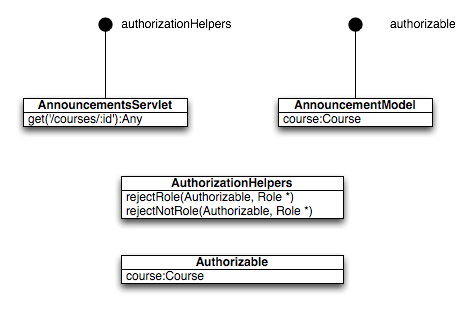
\includegraphics[width=\textwidth]{auth_uml}
\caption{Class Diagram of the Participants in the Authorization System}
\label{fig:auth_uml}
\end{figure}

% subsection authentication (end)

% subsection access_control (end)

\subsection{Realtime(ish)} % (fold)
\label{sub:realtime}

[Overview of methods of realtime, polling, long polling, JSONp, COMET - discussion of Bayeux solution]

% subsection realtime (end)

% section aristotle (end)

\section{Clients} % (fold)
\label{sec:clients}

[Overview of overall client responsibilities]

\subsection{Darkhorse - an HTML5 browser based client} % (fold)
\label{sub:darkhorse}

[Discussion of the benefits of a single page application, local storage cacheing, issues with performance and backwards compatibility ]

% subsection darkhorse (end)

\subsection{Socrates - an iOS client} % (fold)
\label{sub:socrates}

[Simple demonstration of the client server working well, iOS implementation specifics not especially relevant]

% subsection socrates (end)

\subsection{Aristophanes - an Android client} % (fold)
\label{sub:aristophanes}

[Similar to above, illustrate the feasibility of android deployment ]

% subsection aristophanes (end)

\subsection{Plato - a ruby on rails static client} % (fold)
\label{sub:plato}

The Plato app was a small project to briefly experiment with allowing users to run small courses using the Matygo LMS. It served as a marketplace for professionals to sell sessions to small groups of interested learners. It is mentioned in this document only to demonstrate additional development of clients which were powered by the Aristotle API.

Plato is a Ruby on Rails application, which communicates with the Aristotle API by way of a lightweight wrapper around the Ruby Net::Http library which returns custom objects which implement the key ActiveModel interfaces [CITATION NEEDED] allowing Aristotle to act as a data source for the Ruby on Rails web application framework. This decision was made to improve developer efficiency. 

[Generate a Figure showing the interactions between an AR object and the API wrapper]
% subsection plato (end)

% section clients (end)

\section{Operations} % (fold)
\label{sec:operations}

\subsection{Load Balancing} % (fold)
\label{sub:load_balancing}

[More of an academic discussion with respect to our system as it only ever ran on a single box, but was designed with modularity in mind so discuss that arcietecture, nginx reverse proxing]

% subsection load_balancing (end)

\subsection{Continuous Integration and Deployment} % (fold)
\label{sub:continuous_integration_and_deployment}

[Ops system, for simple redeployment, worthy of discussion as operating a large system is a pain, and there are some good bits in here]

% subsection continuous_integration_and_deployment (end)

\subsection{Content Distribution Schemes} % (fold)
\label{sub:content_distribution_schemes}

[Faster page loads around the world with CDN, obvious, but interesting as well. Used to cache dynamicly generated images as well]

% subsection content_distribution_schemes (end)

\subsection{Versioning} % (fold)
\label{sub:versioning}

[Once API is live, and there are clients on devices iPhone / android deveolping a versioning system is needed to prevent existing install failure]

% subsection versioning (end)

% section operations (end)

\bibliography{report}

\end{document}